% !TEX TS-program = xelatex
\documentclass[]{friggeri-cv}

\usepackage{color}
\usepackage{xcolor}
\usepackage{hyperref}
\usepackage{fancyhdr}
\usepackage{pgf-pie}
\usepackage{afterpage}
\usepackage{tikz}
\usepackage{nopageno}
\addbibresource{bibliography.bib}

\RequirePackage{xcolor}
\definecolor{poarange}{HTML}{FF3F00}
\definecolor{orange}{HTML}{FF7309}
\definecolor{red}{HTML}{FF2A09}
\definecolor{dred}{HTML}{7F1500}
\definecolor{dblue}{HTML}{005E7A}
\definecolor{xred}{RGB}{255, 42, 9}
\definecolor{bgreen1}{HTML}{09CFA5}
\definecolor{bgreen2}{HTML}{59B3FF}
\definecolor{white}{HTML}{FFFFFF}

\hypersetup{
	unicode=true,
	pdftoolbar=false,
	pdffitwindow=true,
	pdftitle={Derek Strasters Resume}, 
	pdfauthor={Derek Strasters}, 
	pdfsubject={Resume}, 
	pdfkeywords={Obviously the Best Candidate},
	colorlinks=true,
	urlcolor=dblue
}

 ABCDEFGHIJKLMNOPQRSTUVWXYZ
\ABCDEFGHIJKLMNOPQRSTUVWXYZ
 abcdefghijklmnopqrstuvwxyz
\abcdefghijklmnopqrstuvwxyz
 1234567890.:,; < > (*!?') [1!iIl|]{oO0}
\1234567890.:,; < > (*!?') [1!iIl|]{oO0}\)
 The quick brown fox jumps over the lazy dog.
\The\quick\brown\fox\jumps\over\the\lazy\dog.1

\pagestyle{fancy}

\begin{document}

\rfoot{\scriptsize{This resumé was written in  }\small{\LaTeX}\scriptsize{, the source code may be found on my aforementioned GIT repository.\\Credit to Adrien Friggeri for the \texttt{documentclass} used herein; provided at sharelatex.com}}

\pagenumbering{none}
\header{Derek}{Strasters}
{\{Software\_Engineer\}}

% Fake text to add separator
\fcolorbox{white}{gray}{\parbox{\dimexpr\textwidth-2\fboxsep-2\fboxrule}{%
.....
}}

% In the aside, each new line forces a line break
\begin{aside}
	\section{Cellphone} 
	(801) 580 - 5293
	~
	\section{Mail}
		\href{mailto:paracite.org@gmail.com}{\textbf{paracite.org@}\\gmail.com}
		\href{mailto:D.Strasters@utah.edu}{\textbf{D.Strasters@}\\utah.edu}
		~
	\section{Web \& Git}
		\href{http://paracite.org/portfolio}{\textbf{paracite.org}}
		\href{https://github.com/thehumanparacite}{github.org/\\ \textbf{thehumanparacite}}
		~
	\section{Address}
	226 E. Kelsey Ave.
	84111 SLC, Utah
	~ 
	\section{Programming}
	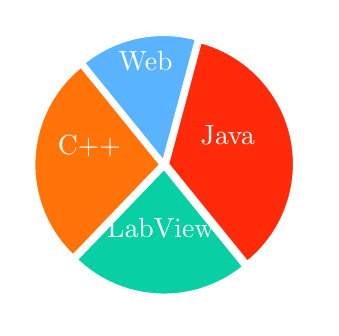
\begin{tikzpicture}
		\color{white}
		\pie[%
				before number={\hphantom},%
				after number=,%
				explode=0.05,%
				color={bgreen2,orange,bgreen1,red},%
				radius=1.6,%
				text=inside,%
				rotate=75]%
			{15/ Web, 27/ C++, 23/ LabView, 35/ Java}
	\end{tikzpicture}
	~
	\section{OS Preference}
		\textbf{Linux}\includegraphics[scale=0.40]{img/5stars.png}
		\textbf{Windows}\includegraphics[scale=0.40]{img/4stars.png}
		\textbf{MacOS}\includegraphics[scale=0.40]{img/2stars.png}
		~
	\section{Personal Skills}
	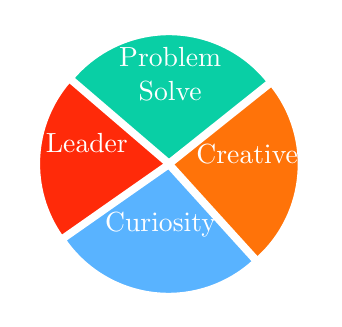
\begin{tikzpicture}
		\color{white}
			\pie[%
					before number={\hphantom},%
					after number={},%
					explode=0.05,%
					color={bgreen2,orange,bgreen1,red},%
					radius=1.6,%
					text=inside,%
					rotate=215]%
				{27/ Curiosity, 24/ Creative, 28/ Problem\\ Solve, 21/ Leader}
		 
	\end{tikzpicture}
	~
\end{aside}

\section{Experience}
\begin{entrylist}
	\entry
		{11/14 - [now]}
		{Senior Developer \& Co-Founder}
		{Snicker Media Inc.}
		{•Lead developer of Android app, \href{http://isnicker.com/}{\textbf{SnicKer}}, a socially driven image sharing app\\ 
		•Heavy use of \href{https://en.wikipedia.org/wiki/OAuth}{\textbf{OAuth}} integration for sharing on other social media networks\\ }
	\entry
		{03/13 - 07/15}
		{Mechanical Engineer Tech.}
		{BioFire Diagnostics}
		{•Integral role in creating company coding guidelines for PLC unit programming\\
		•Design of \href{http://www.biomerieux-diagnostics.com/filmarray-multiplex-pcr-system}{medical} manufacturing systems involving high vacuum, heat, and motion\\
		Programmed and managed CNC machining center for manufacturing R&D parts\\} 
	\entry
		{12/09 - 06/09}
		{Solid State Research}
		{University of Utah}
		{Developed robust data \href{http://www.ni.com/data-acquisition/what-is/}{\textbf{acquisition}} software.\\  
		Designed electronics and circuitry for data acquisition instrumentation.\\
		Developed specialized data \href{https://en.wikipedia.org/wiki/Data_analysis}{\textbf{analysis}} software.\\
		Experience with electron microscopy and E-beam lithography.\\  
		Emphasis of research was on organic semiconductors.}
\end{entrylist}

\section{Achievements}
\begin{entrylist}
	\entry
		{\hphantom{1234}2015} % FIXME: Get rid of hacky solution to spacing 
		{Neural Net Framework}
		{Personal}
		{Highly customizable \href{https://en.wikipedia.org/wiki/Artificial_neural_network}{\textbf{neural network}} written in C++ 98. What started as a school project has led to this, my personal favorite creation. The code is available for review in my \href{https://github.com/TheHumanParacite/SeaPlusPlus-Projects/tree/master/NeuralNet}{\textbf{git repository}} and will compile on most standard Linux distributions.\\}
	\entry
		{\hphantom{1234}2012}
		{Android}
		{Symbol Buddy}
		{Developed study aid for students of Physics and Math.\\
		Found on Google Play under the name \href{https://play.google.com/store/apps/details?id=org.paracite.symbolbuddy}{\textbf{Symbol Buddy}}.\\}
	\entry
		{\hphantom{1234}2014}
		{Certified SolidWorks Professional}
		{DS SolidWorks Corp.}
		{Certification done through Dassault's official on-line testing programme.\\ 
		Certificate may be viewed using ID number \href{https://solidworks.virtualtester.com/validate_button}{\textbf{c-tmhwzetlwy}}.\\}
		
\end{entrylist}

\section{Education}
\begin{entrylist}
	\entry
		{2010 - \hphantom{12}now}
		{Bachelors in Physics (in progress)}
		{University of Utah}
		{\textbf{[only 4 credit hours remain from completion]}\\
		Areas of Strength: Electronics, Computational Physics, and Data Acquisition\\
		Highly experienced in research lab setting (see above).\\
		{\emph{Head of Lab Group: Prof. Andrey Rogachev of University of Utah}\\}}		

\end{entrylist}
\end{document}
